\documentclass[11pt]{article} % scrbook otro formato
\usepackage[utf8]{inputenc}
\usepackage[spanish,es-tabla,es-nodecimaldot]{babel}

% Paquetes

\usepackage{amsmath}
\usepackage{amsthm}
\usepackage{amsfonts}
\usepackage{amssymb}
\usepackage{makeidx}
\usepackage{graphicx}
\usepackage{lmodern}
%\usepackage{kpfonts}
\usepackage{fancyhdr}
\usepackage{geometry}
\usepackage{lastpage}
\usepackage{array} % Para fjar tamaño de columnas
\RequirePackage{siunitx}
\RequirePackage{tcolorbox}
\usepackage{extramarks} % Para poder usar firstleftmarks
\usepackage[version=4]{mhchem} % Para poder usar formulas de reacciones nucleares
\usepackage{xcolor}
\usepackage{booktabs}
%\usepackage{newtxtext, newtxmath} % Cambia la fuente (pero mola)

\newtcolorbox{mybox}{colback=black!5!white,
	colframe=black!75!black}
\newtcolorbox{mybox2}{colback=blue!5!white,
	colframe=black!75!black}



%##############################################################################
%######### Ponemos el decimal con . ###########################################
%##############################################################################

\sisetup{output-decimal-marker={.},
	% exponentes ------------------------
	%exponent-mode=threshold,
	%exponent-thresholds=-3:2, % non usar exponentes 10^{-2,-1, 0, 1}
	% redondear -------------------------
	% round-mode=figures, % cifras sig
	% round-mode=places, % cantos decimales
	round-mode=uncertainty, % cifras sig da incerteza (necesario usar erro)
	round-precision=2,
	uncertainty-mode = separate,
	print-unity-mantissa=false,
	% unidades --------------------------
	inter-unit-product = \ensuremath{{}\cdot{}}, % separacion entre unidades
	% per-mode=power-positive-first, % so furrula con metodo interpretado puro
	inline-per-mode=single-symbol,
	display-per-mode=fraction,
}

%##############################################################################
%######### Para codigo python #################################################
%##############################################################################

\definecolor{codegreen}{rgb}{0,0.6,0}
\definecolor{codegray}{rgb}{0.5,0.5,0.5}
\definecolor{codepurple}{rgb}{0.58,0,0.82}
\definecolor{backcolour}{rgb}{0.95,0.95,0.92}

\usepackage{listings}


%\lstdefinestyle{mystyle}{	backgroundcolor=\color{backcolour},   	commentstyle=\color{codegreen},	keywordstyle=\color{magenta},	numberstyle=\tiny\color{codegray},	stringstyle=\color{codepurple},	basicstyle=\ttfamily\footnotesize,	breakatwhitespace=false,         	breaklines=true,                 	captionpos=b,                    	keepspaces=true,                 	numbers=left,                    	numbersep=5pt,                  	showspaces=false,                	showstringspaces=false,	showtabs=false,                  	tabsize=2}

%\lstset{style=mystyle}
%\usepackage{background}     % Para manejar el fondo


%##############################################################################
%######### Tipo de fuente #################################################
%##############################################################################

%\usepackage{kpfonts}

%\usepackage{helvet} 
%\renewcommand{\familydefault}{\sfdefault}.

%\usepackage{fontspec} % Paquete necesario para seleccionar fuentes
%\setmainfont{Verdana} % Cambia la fuente principal a Verdana


%##############################################################################
%######### Geometría #################################################
%##############################################################################

\geometry{a4paper, total={152mm,237mm}, left=31mm, top=30mm}





%##############################################################################
%######### Formatos capítulo #################################################
%##############################################################################

%\usepackage[lmodern]{quotchap}
%\usepackage[Bjornstrup]{fncychap}

% Para el Bjornstrup
%\ChNumVar{\fontsize{76}{80}\usefont{OT1}{pzc}{m}{n}\selectfont}
%\ChTitleVar{\raggedright\Huge\sffamily\bfseries}


%##############################################################################
%######### Hiperreferenias #################################################
%##############################################################################


\usepackage[colorlinks=true,allcolors=blue]{hyperref} % Crea las


%##############################################################################
%######### Formato de pagina #################################################
%##############################################################################

%\renewcommand{\chaptermark}[1]{\markboth{\chaptername\ \thechapter.\ #1}{}}
\renewcommand{\sectionmark}[1]{\markright{\thesection.\ #1}}

\setlength{\headsep}{27pt} % Distancia entre la cabezera y el texto
\setlength{\footskip}{30pt} % Distancia entre el pie de pagina y el texto
\pagestyle{fancy}
\fancyhf{}
\fancyhead[LE]{\rightmark} % L,R,C-> left, right, center [LE,RO]
\fancyhead[RO]{\rightmark} % E,O -> even (par), odd (impar)
\fancyhead[LO,RE]{Daniel Vázquez Lago}
\fancyfoot[CE,CO]{\thepage}
\renewcommand{\headrulewidth}{1pt} % Cambiamos el grosor de la linea de arriba
\renewcommand{\footrulewidth}{0pt}



%##############################################################################
%#########  Modificar caption #################################################
%##############################################################################

\usepackage[font=small, justification=centering]{caption}  % Configura las captions



%##############################################################################
%######### Comandos propios #################################################
%##############################################################################

\newcommand{\parentesis}[1]{\left( #1  \right)} 
\newcommand{\parciales}[2]{\frac{\partial #1}{\partial #2}}
\newcommand{\pparciales}[2]{\parentesis{\parciales{#1}{#2}}}
\newcommand{\ccorchetes}[1]{\left[ #1  \right]}
\newcommand{\D}{\mathrm{d}}
\newcommand{\derivadas}[2]{\frac{\D #1}{\D #2}}

\newcommand{\tquad}{\quad \quad \quad}
\newcommand{\dquad}{\quad \quad}
\newcommand{\vnabla}{\vec{\nabla}}

\newcommand{\Acal}{\mathcal{A}}
\newcommand{\Ocal}{\mathcal{O}}
\newcommand{\Ncal}{\mathcal{N}}
\newcommand{\Hcal}{\mathcal{H}}
\newcommand{\Ucal}{\mathcal{U}}
\newcommand{\Lcal}{\mathcal{L}}

\newcommand{\logd}{\log_{10}}

\newcommand{\eV}{\text{eV}}
\newcommand{\cm}{\text{cm}}
\newcommand{\cmm}{\text{cm}^{-1}}
\newcommand{\fm}{\text{fm}}
\newcommand{\He}{\text{He}}
\newcommand{\p}{\text{p}}
\newcommand{\e}{\text{e}}
\newcommand{\cte}{\text{cte}}


% Comandos vectoriales

\newcommand{\an}{\mathbf{a}}
\newcommand{\bn}{\mathbf{b}}
\newcommand{\dn}{\mathbf{d}}
\newcommand{\jn}{\mathbf{j}}
\newcommand{\lnn}{\boldsymbol{\ell}}
\newcommand{\lnnn}{\boldsymbol{l}}
\newcommand{\kn}{\mathbf{k}}
\newcommand{\pn}{\mathbf{p}}
\newcommand{\qn}{\mathbf{q}}
\newcommand{\rn}{\mathbf{r}}
\newcommand{\sn}{\mathbf{s}}
\newcommand{\un}{\mathbf{u}}
\newcommand{\vn}{\mathbf{v}}
\newcommand{\xn}{\mathbf{x}}
\newcommand{\yn}{\mathbf{y}}
\newcommand{\qndot}{\dot{\qn}}

\newcommand{\unovec}{\vec{\mathbf{1}}}

\newcommand{\alphan}{\boldsymbol{\alpha}}
\newcommand{\sigman}{\boldsymbol{\sigma}}
\newcommand{\pin}{\boldsymbol{\pi}}


\newcommand{\An}{\mathbf{A}}
\newcommand{\Bn}{\mathbf{B}}
\newcommand{\En}{\mathbf{E}}
\newcommand{\Gn}{\mathbf{G}}
\newcommand{\Jn}{\mathbf{J}}
\newcommand{\Kn}{\mathbf{K}}
\newcommand{\Ln}{\mathbf{L}}
\newcommand{\Rn}{\mathbf{R}}
\newcommand{\Sn}{\mathbf{S}}
\newcommand{\Tn}{\mathbf{T}}
\newcommand{\In}{\mathbf{I}}

\newcommand{\hnn}{\hat{\mathbf{n}}}
\newcommand{\hnr}{\hat{\mathbf{r}}}
\newcommand{\hnz}{\hat{\mathbf{z}}}
\newcommand{\hnx}{\hat{\mathbf{x}}}
\newcommand{\hny}{\hat{\mathbf{y}}}
\newcommand{\hnu}{\hat{\mathbf{u}}}
\newcommand{\hnR}{\hat{\mathbf{R}}}
\newcommand{\hnv}{\hat{\mathbf{v}}}
\newcommand{\hnk}{\hat{\mathbf{k}}}
\newcommand{\hni}{\hat{\mathbf{i}}}
\newcommand{\hnj}{\hat{\mathbf{j}}}
\renewcommand{\hnk}{\hat{\mathbf{k}}}

\newcommand{\Ec}{\langle E_c \rangle}
\newcommand{\Ecinv}{\langle E_c^{-1} \rangle}
\newcommand{\varphiV}{\langle \varphi_V \rangle}
\newcommand{\varphiVV}{\langle \varphi_{VV}\rangle}
\newcommand{\varphiVEcinv}{\langle \varphi_V E_c^{-1} \rangle}
\newcommand{\varphiVVEcinv}{ \langle \varphi_V^2 E_c^{-1} \rangle}

%##############################################################################
%######### Teoremas/definiciones #################################################
%##############################################################################

%\theoremstyle{definition}
%\newtheorem{definition}{Definición}[chapter]
%\theoremstyle{theorem}
%\newtheorem{theorem}{Teorema}[chapter]




%##############################################################################
%######### Referncia para euccaiones y figuras ################################
%##############################################################################

%\numberwithin{equation}{section}
%\numberwithin{figure}{section}




%##############################################################################
%######### Documento #################################################
%##############################################################################


\author{Daniel Vazquez Lago}
\title{Simulación en física de materiales}


\begin{document}	
	
\maketitle
\newpage
\tableofcontents
	
\setlength{\parskip}{1.5mm} % Cambia el espacio entre párrafos
	
\section{Objetivos}	

En este optativo nuestro objetivo principal es obtener algunas de las propiedades estáticas y dinámicas a partir de la posición y velocidad en diferentes instantes de tiempo obtenidas en el ejercicio anterior de dinámica molecular para la colectividad microcanónica. Primero veremos como obtenerlas teóricamente, para luego mostrar los resultados obtenidos a partir de la simulación. 

Es muy importante mencionar que en nuestro caso, como usamos variables reducidas, la densidad másica, generalmente denotada por $\rho$, es igual a la densidad de partículas, que se suele expresar como $n$. Nosotros usaremos $\rho$ en vez de $n$ para hablar de densidad de partículas.

\section{Teoría}

\subsection{Propiedades estáticas: distribución radial}

En realidad ya hemos calculado algunas propiedades estáticas en el obligatorio 3: la presión, la capacidad calorífica a volumen constante... es decir, todas las propiedades termodinámicas son propiedades estáticas, que por ejemplo también podemos obtener con Monte-Carlo (aunque no en la colectividad microcanónica). 

En esta sección vamos a tratar con la estructura de nuestro gas, que puede ser obtenida a partir de la \textbf{distribución radial} $g(r)$. Esta función nos da información acerca de como las moléculas se organizan alrededor de otro, es decir, como es la <<estructura local>>. Específicamente, es proporcional a la probabilidad de encontrar dos átomos separados por una distancia $r\pm \Delta r$, y juega un papel fundamental en la mecánica estadística de sustancias densas. Como la dinámica molecular nos da las posiciones de los átomos individuales, es muy sencillo obtener $g(r)$. La función de distribución radial depende de la densidad y la temperatura, y es un indicador para saber la fase en la que se encuentra el sistema simulado \cite{Haile}.



\subsection{Propiedades dinámicas: coeficientes de difusión}

Denominamos como difusión al proceso por el cual un sistema de partículas iniciales pasan de una configuración inicial no uniforme a otra configuración sin una corriente, solo por el movimiento de las partículas en el fluido. Macroscópicametne la ley que describe la difusión es la \textit{ley de Flick} \cite{Frenkel}, que define un parámetro único para cada fluido llamado \textbf{coeficiente de difusión} $D$. Esta ley nos dice que la velocidad de los elementos continuos $\vn$ está relacionada con el gradiente de la densidad tal que \cite{Rapaport}

\begin{equation}
	\rho \vn  = - D \nabla \rho
\end{equation}
Como sabemos la \textit{ecuación de continuidad de la masa} nos exige que

\begin{equation}
	\parciales{\rho}{t} = - \nabla (\vn \rho)
\end{equation}
de tal modo que 

\begin{equation}
	\parciales{\rho}{t} = D \nabla^2 \rho
\end{equation}
Una solución para nuestro sistema podría ser \cite{Frenkel}: 

\begin{equation}
	\rho (r,t) = \frac{1}{(4\pi Dt)^{3/2}} \exp \parentesis{- \frac{r^2}{4Dt}}
\end{equation}
Ahora nos preguntamos: ¿Cómo podemos obtenemos $D$ a partir de estas ecuaciones? Existen dos maneras: a través del \textit{desplazamiento cuadrático medio} y a través de la \textit{correlación de velocidad}, tal y como vamos a ver a continuación. 

\subsubsection{Desplazamiento cuadrático medio}

Dado que en el instante $t=0$ la densidad sigue una delta de Dirac $\rho(\rn,t)=\delta(\rn)$, en dicho instante todas las partículas se van a encontrar en $r=0$. Es evidente entonces que el  \textbf{desplazamiento cuadrático medio} $\langle (\rn(t)-\rn(0))^2 \rangle$ vendrá dado por \cite{Haile}:

\begin{equation}
	\langle (\rn(t)-\rn(0))^2 \rangle  = \frac{1}{\rho} \int \rn^2 \rho(\rn,t)\D^3 \rn
\end{equation}
Lo cual nos lleva, resolviendo la integral

\begin{equation}
	6Dt = \langle (\rn(t)-\rn(0))^2 \rangle
\end{equation}
Este resultado sólo es válido cuando $t$ es más grande que el tiempo entre colisión de los átomos \cite{Haile} por lo que de manera más exacta el coeficiente de difusión viene dado por:

\begin{equation}
D = \frac{1}{6} \lim_{t\rightarrow\infty} \frac{\langle (\rn(t)-\rn(0))^2 \rangle}{t}
\end{equation}


\subsubsection{Correlación de velocidad}

El cálculo de la difusión a través de la correlación de las velocidades se hace a través de las relaciones de Green-Kubo, que en general se deducen para una propiedad dinámica cualquiera $A(t)$ \cite{Haile}, aunque nosotros ya vamos a particularizar el resultado siendo la propiedad dinámica la posición de las partículas. Tenemos que 

\begin{equation}
	\vn=\dot{\rn}(t) = \derivadas{\rn}{t}
\end{equation} 
tal que
\begin{equation}
	\rn(t)-\rn(0) = \int_{0}^{t} \vn(\tau) \D \tau
\end{equation}
Elevando el cuadrado y haciendo el valor medio sobre obtenemos el desplazamiento cuadrático medio en función de 

\begin{equation}
	\langle	(\rn(t)-\rn(0))^2 \rangle = \int_{0}^{t}\D \tau' \int_{0}^{t}  \D \tau''  \langle \langle	\vn(\tau') \vn(\tau'') \rangle 
\end{equation}
Como podemos ver estamos integrando sobre un <<cuadrado de superficie $t^2$>> en el espacio simétrico $\tau'-\tau''$. El mismo valor se obtiene si integramos sobre un <<triángulo de este cuadrado y lo multiplicamos por dos>>, tal que:

\begin{equation}
	\langle	(\rn(t)-\rn(0))^2 \rangle = 2 \int_{0}^{t} \D \tau''\int_{0}^{\tau''} \D \tau'   \langle \langle	\vn(\tau''-\tau') \vn(0) \rangle 
\end{equation}
Siempre podemos hacer el cambio de variables $\tau=\tau''-\tau'$ tal que 

\begin{equation}
	\langle	(\rn(t)-\rn(0))^2 \rangle = \int_{0}^{t}\D \tau'' \int_{0}^{\tau''} \D \tau  \langle \langle	\vn(\tau) \vn(0) \rangle 
\end{equation}
Sin embargo la integral es invariante si hacemos el cambio de límites, tal que


\begin{equation}
	\langle	(\rn(t)-\rn(0))^2 \rangle = 2 \int_{0}^{t}\D \tau   \langle \langle	\vn(\tau) \vn(0) \rangle \int_{\tau}^{t} \D \tau''
\end{equation}
y ahora:

\begin{equation}
	\langle	(\rn(t)-\rn(0))^2 \rangle = 2t \int_{0}^{t}\D \tau   \langle \langle	\vn(\tau) \vn(0) \rangle \parentesis{1-\frac{\tau}{t}}
\end{equation}
y si $t\rightarrow\infty$ a ambos lados:

\begin{equation}
	\lim_{t\rightarrow\infty} \frac{ \langle	(\rn(t)-\rn(0))^2 \rangle}{2t} = \lim_{t\rightarrow\infty}   \int_{0}^{t}\D \tau   \langle \langle	\vn(\tau) \vn(0) \rangle \parentesis{1-\frac{\tau}{t}}
\end{equation}
nos lleva directamente a que

\begin{equation}
	D = \frac{1}{3} \int_0^\infty \langle v(t)v(0)\rangle \D \tau
\end{equation}
es decir, hemos obtenido $D$ en función de la correlación de las velocidades $\langle v(t)v(0)\rangle$.

\section{Implementación}

Hemos visto en la sección anterior como se define la función de distribución radial y como se obtiene el coeficiente de difusión $D$ teóricamente. En esta sección veremos como podemos implementar las ecuaciones anteriores de manera práctica en nuestra simulación a partir de los datos que tenemos: posiciones y velocidades de las 500 partículas para 5000 configuraciones temporales diferentes con una distancia de $\Delta t = 0.01$. 

\subsection{Obtención de la función de distribución radial}

Existen varias formas de calcular la función de distribución radial, y nosotros usaremos la más sencilla de todas. Para una configuración instantánea de $N$ partículas  obtener las $N(N-1)$ distancias es bastante sencillo, basta con usar un bucle que recorra cada una de las partículas, que a su vez contenga otro bucle que recorra las N-1 partículas restantes. Dado que las distancias van a pares (la distancia de $i$ a $j$ es la misma que de $j$ a $i$), podemos reducir el número de interacciones a la mitad. 

Una vez tentemos los $N(N-1)/2$ pares de distancias podremos asignar cada una de estas a un bin de un histograma. Cuando esta distancia caiga en el intervalo  $r+\Delta r$ aumentaremos en 2 la frecuencia de dicho intervalo. Elegir un tamaño adecuada para la anchura del intervalo $\Delta r$ es un ejercicio complicado, ya que una anchura pequeña aumenta la resolución pero también aumenta el error estadístico (proporcional a $1/\sqrt{\Delta r}$) \cite{Frenkel}. También hay que tener en cuenta que debido a que usamos condiciones de contorno periódicas la distancia máxima a la que podremos evaluar la función de distribución radial es $r_c$ (en nuestro caso $r_c=5$). La anchura será entonces $r_c/1000$, es decir $\Delta r=0.005$.


\begin{figure}[h!] \centering
	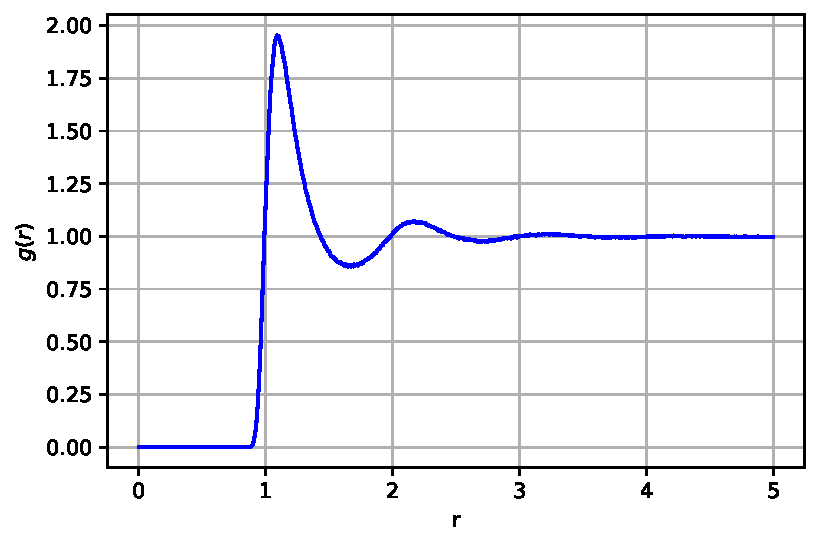
\includegraphics[width=0.65\textwidth]{../../Graficas/Optativo2/gr.pdf}
	\caption{Gráfico de la distribución radial}
	\label{Fig:01}
\end{figure}

Si suponemos que el número de pares del intervalo $\{ r, r+\Delta r\}$ es $N_p$ y $\langle N_p^{\text{id}} \rangle$ es el número de partículas que encontraríamos en el mismo rango pero para un gas ideal, tenemos que:

\begin{equation}
	g(r) = \frac{\langle N_p (r)\rangle}{N_p^{\text{id}}(r)}
\end{equation}
donde $N_p^{\text{id}}(r)=\frac{1}{2} N \rho (4 \pi/3) [(r+\Delta r)^3-r^3]$. Dado que nosotros tenemos 5000 configuraciones instantáneas, los valores de la distribución radial será un promedio de dichas 5000 configuraciones, para así minimizar el error estadístico. En la figura \ref{Fig:01} podemos ver una de las configuraciones para el conjunto de las 5000 configuraciones (hay que tener en cuenta que tenemos 10 de estas, y por tanto 10 gráficas de distribución radial).


\subsection[Coeficiente de difusión a través de $d_{cm}$]{Cálculo del coeficiente de difusión a través del desplazamiento cuadrático medio}

El desplazamiento cuadrático medio denotado por $d_{cm}$ de una configuración $\tau$ respecto una configuración en el instante $\tau_0$ es:

\begin{equation}
		d_{cm}(\tau,\tau_0)=\langle (\rn(\tau)-\rn(\tau_0))^2 \rangle = \sum_{i=1}^N (\rn_i(\tau)-\rn_i(\tau_0))^2  
\end{equation}
Como hemos visto no importa el instante $\tau$ y $\tau_0$ sino la diferencia temporal $t=\tau-\tau_0$. En el apartado teórico hemos visto que

\begin{equation}
	d_{cm} (t)= 6D t
\end{equation}
entonces si representamos $d_{cm}$ frente a $t$ la gráfica debería ser lineal para $t$ mucho mayores que la tasa de colisión (es decir, $t$ grande). Entonces si representamos $D(t)$ frente a $t$ y hacemos la regresión lineal solo en la parte que tiene un comportamiento lineal podremos obtener el valor del coeficiente de difusión. Si representamos $d_{cm}$ frente a $t$ a partir del primer instante de la configuración podríamos evaluar hasta $t=50$. Sin embargo, no es necesario, ya que el comportamiento lineal aparece ya bastante pronto ($t=1.5$) y se obtiene un buen coeficiente de difusión con una regresión lineal con datos hasta $t=3$.

\begin{figure}[h!] \centering
	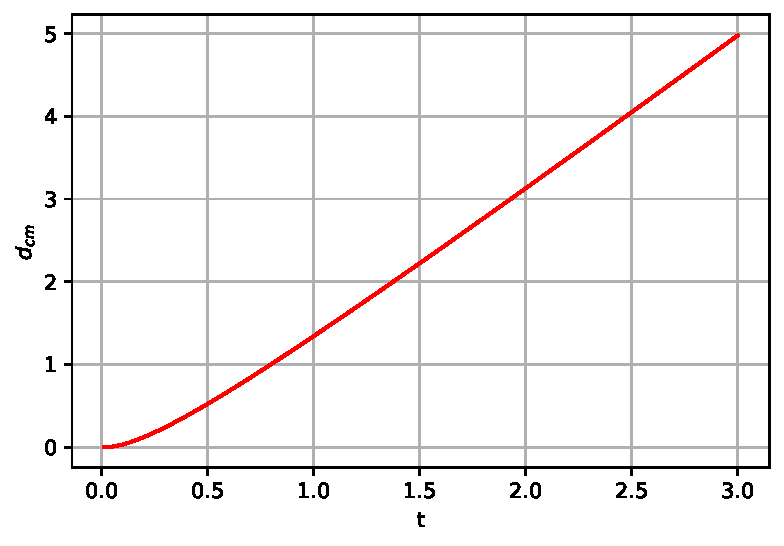
\includegraphics[width=0.65\textwidth]{../../Graficas/Optativo2/dcm2.pdf}
	\caption{Gráfico del desplazamiento cuadrático medio con el tiempo.}
	\label{Fig:02}
\end{figure}

Como tenemos hasta $t=50$, lo que podemos hacer es coger diferentes $\tau_0$ y calcular hasta $\tau=\tau_0+3$, de tal modo que tengamos varios diferentes del desplazamiento cuadrático medio para cada $t\in[0,3]$, de tal modo que podamos hacer un promedio y minimizar el error estadístico. De esta manera hemos obtenido la imagen \ref{Fig:02}, en la que se puede ver un comportamiento lineal a partir de $t=1.5$, tal y como habíamos dicho. Los resultados para cada una de los 500K los podemos ver en la tabla \ref{Tab:02}, y el resultado medio (e incertidumbre) en la tabla \ref{Tab:01}. Al igual que en el ejercicio anterior, suponemos que cada uno de estos 500K pasos son un <<experimento independiente>> aunque en realidad formen parte de la misma simulación, para poder darle así una incertidumbre a los valores medios obtenidos a través de la simulación.



\subsection[Coeficiente de difusión a través de $\text{Corr}_v$]{Cálculo del coeficiente de difusión a través de la correlación de velocidades}

El coeficiente de difusión a través de la correlación de velocidades exige dos puntos: convertir la integral en un sumatorio finito y convertir el valor medio como la suma sobre las partículas. Así tenemos que 


\begin{equation}
	\text{Corr}_v(t)\equiv \langle v(t)v(0)\rangle = \sum_{i}^N \vn_i(t) \cdot \vn_i(0)
\end{equation}
tal que 
\begin{equation}
	D = \frac{1}{3} \sum_{k=0}^{k_{\max}}  \text{Corr}_v (k \cdot \Delta t) \Delta t
\end{equation}
Al igual que en el cálculo del coeficiente de difusión integraremos hasta $t=3$, ya que a partir de este instante el valor de la correlación cae a cero ($\sim 10^{-3}$. Consecuentemente, e igual que antes, de esta forma podemos obtener varios valore para cada $t\in[0,3]$ de tal manera que podamos hacer un promedio y minimizar el error estadístico.

En la gráfica \ref{Fig:02} hemos representado el valor de $\text{Corr}_v$ para diferentes $t$, de tal manera que efectivamente podemos ver como al principio la correlación es muy grande pero cae rápidamente para tener un valor relativo muy pequeño en $t=3$ (unos 3 órdenes de magnitud diferentes). Los datos obtenidos en cada una de las 500K interacciones están en la tabla \ref{Tab:02}, y la media con su incertidumbre está en \ref{Tab:01}.


\begin{figure}[h!] \centering
	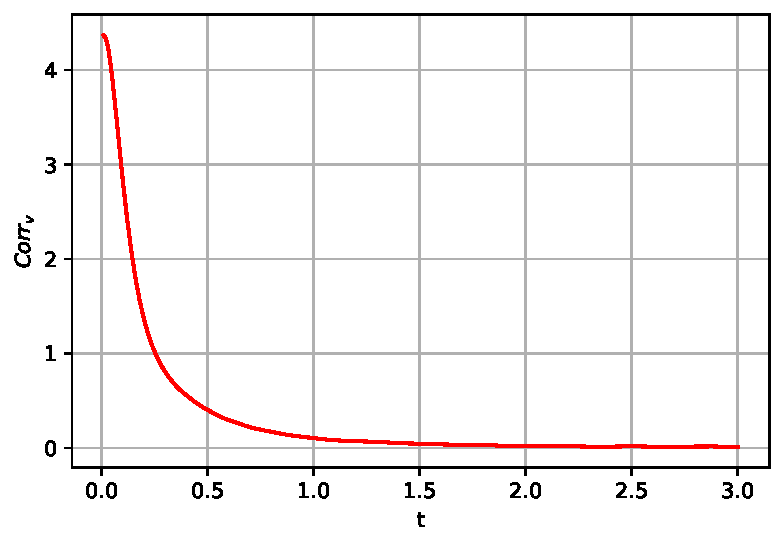
\includegraphics[width=0.6\textwidth]{../../Graficas/Optativo2/Corr_vel.pdf}
	\caption{Gráfico de correlación de la velocidad con el tiempo.}
\end{figure}


\section{Organización} \label{Sec:05}

En esta sección mencionare como están organizados el proyecto. En primer lugar hay que decir que, por motivos de organización personal, he creado una carpeta llamada \textit{Datos} donde se almacenan todos los \texttt{.dat} de todos los proyectos. Sin embargo para que se guarden correctamente he supuesto que se ejecuta desde el proyecto, esto es, desde el \texttt{.exe} que se genera al construir el proyecto. De hacerlo de otro modo esto llevaría a un error. Una breve descripción de los archivos:

\begin{itemize}
	\item \textbf{Optativo\_2}: programa principal en el que se leen los datos generados por la dinámica molecular obteniendo las propiedades dinámicas. Este programa pide a teclado cual de los 10 archivos lee, generado el archivo de datos que contiene la correlación de velocidades y desplazamiento cuadrático medio para el mismo. 
	\item \textbf{Optativo\_2\_g}: programa principal en el que se leen los datos generados por la dinámica molecular obteniendo la función radial. Este programa pide a teclado cual de los 10 archivos lee, generado el archivo que contiene el archivo de la función de distribución radial para el mismo.
\end{itemize}
Además también usamos dos archivo a lotes (\texttt{.bat})

\begin{itemize}
	\item \textbf{Ejectuta\_Optativo\_2}: en este archivo de lotes es en el que realmente ejecutamos ejecutamos el \texttt{Optativo\_2}, ejecutando el \texttt{.exe} un cierto número de veces (10 en principio) escribiendo el valor de entrada que necesita para leer el archivo. 
	\item \textbf{Ejectuta\_Optativo\_2\_g}: en este archivo de lotes es en el que realmente ejecutamos ejecutamos el \texttt{Optativo\_2\_g}, ejecutando el \texttt{.exe} un cierto número de veces (10 en principio) escribiendo el valor de entrada que necesita para leer el archivo. 
\end{itemize}
Y archivos de \texttt{Python} para hacer las gráficas, convertir los datos en tablas de \LaTeX, hacer la integral y obtener los datos de la regresión lineal:

\begin{itemize}
	\item \textbf{Opt\_02}: en este archivo de Python leemos los datos generados por los dos programas principales, de tal manera que hace las gráficas, la regresión lineal (a través del módulo Scipy) y calcula la integral para cada uno de los valores.
\end{itemize}


\section{Conclusiones}

Una vez creado y ejecutado los programas obtenemos las gráficas y datos para cada una de las 500K interacciones. En esta sección vamos a ver que información podemos obtener de los datos presentados y un pequeño análisis de los mismos. De la función de distribución radial no podemos obtener mucha información. Lo más interesante sería que a partir de esta calculáramos el factor de estructura, un valor que es muy fácil de obtener experimentalmente a partir de la difracción de rayos x o de neutrones, y así comparando el experimental y el simulado. Sin embargo, los resultados no son presentables, por lo que la única información que podemos sonsacar de esta función es que nuestro gas en realidad está en fase líquida, ya que las oscilaciones respecto $1$ en $r>1$ nos indica cierta presencia de una distribución organizada, propia de un cristal \cite{Haile}.

Los datos presentados para el coeficiente de difusión \ref{Tab:01} son bastante buenos desde un punto de vista estadístico: para uno y otro método el valor no es diferente. Es cierto que existe una diferencia, y, aunque teóricamente no debería existir (ambas dos proceden de la misma ley y por tanto las limitaciones teóricas son las mismas), el carácter finitesimal de las simulaciones hacen que exista, ya que no podemos lleva $t$ al infinito. Esto afecta de manera bastante particular a $D_{corrv}$ ya que estamos limitando una integral que va a infinito a $t<3$, y de manera igual a $D_{dcm}$ ya que el carácter lineal se manifiesta solo en $t\rightarrow\infty$. Además de esto, otras limitaciones serían las inherentes a toda simulación: integrales que son sumatorios, números no reales... además de que los datos de $\rn$ y $\vn$ no son realmente los que siguen las partículas, son simulaciones que contienen errores debido a usar métodos finitos para resolver las ecuaciones diferenciales del movimiento. El error relativo entre uno y otro es menor del 5\% lo cual es satisfactorio, aunque haría falta estudios estadísticos para dilucidar si son compatibles (hipótesis nula).

Como conclusión final podemos decir que aunque los datos extraídos son satisfactorios, haría falta un análisis estadístico más profundo para ver si son compatibles. Además una mayor cantidad de datos o mejora de la simulación (más partículas, caja mas grande) haría que pudiéramos obtener valores concluyentes del factor de forma $S$. Sin embargo, la mejora más evidente es incluir más propiedades dinámicas: conductividad térmica, viscosidades (tensoriales)...
	
\begin{table}[h!] \centering
\begin{tabular}{lrr}
\toprule
Variable & Media & Incertidumbre \\
\midrule
$E_c^*$ & 1093.606 & 1.127 \\
$E_p^*$ & -1668.615 & 1.129 \\
$E_t^*$ & -575.009 & 0.002 \\
$T^*$ & 1.461 & 0.002 \\
$P^*$ & 0.683 & 0.001 \\
$C_V^*$ & 949.116 & 9.003 \\
$\alpha_E^*$ & -9.757 & 0.161 \\
$\gamma^*$ & 0.563 & 0.005 \\
$1/k_s^*$ & 1.537 & 0.004 \\
$k_s^*$ & 0.651 & 0.002 \\
$\alpha_P^*$ & 0.487 & 0.008 \\
$\alpha_S^*$ & -1.216 & 0.012 \\
$1/\alpha_{E2}^*$ & -0.103 & 0.010 \\
$\alpha_{E2}^*$ & -9.737 & 0.985 \\
$1/k_T^*$ & 1.097 & 0.010 \\
$k_T^*$ & 0.911 & 0.008 \\
\bottomrule
\end{tabular}

\caption{Valores del coeficiente de difusión medio e incertidumbre $2\sigma$ de la media para cada método.}
\label{Tab:01}
\end{table}
\begin{table}[h!] \centering
\begin{tabular}{rrrrrrrrr}
\toprule
$E_c^*$ & $E_p^*$ & $E_t^*$ & $T^*$ & $P^*$ & $C_V^*$ & $\alpha_E^*$ & $\gamma^*$ & $1/k_s^*$ \\
\midrule
1093.896 & -1668.904 & -575.008 & 1.461 & 0.684 & 945.430 & -9.911 & 0.564 & 1.540 \\
1095.488 & -1670.502 & -575.013 & 1.464 & 0.684 & 927.931 & -9.579 & 0.575 & 1.544 \\
1092.296 & -1667.301 & -575.004 & 1.459 & 0.682 & 948.219 & -9.886 & 0.562 & 1.532 \\
1096.553 & -1671.567 & -575.014 & 1.465 & 0.685 & 961.826 & -9.908 & 0.555 & 1.538 \\
1091.555 & -1666.562 & -575.007 & 1.458 & 0.682 & 945.798 & -9.215 & 0.569 & 1.542 \\
1091.819 & -1666.827 & -575.007 & 1.459 & 0.682 & 958.523 & -9.635 & 0.559 & 1.531 \\
1093.545 & -1668.554 & -575.009 & 1.461 & 0.683 & 929.783 & -9.801 & 0.573 & 1.540 \\
1095.413 & -1670.424 & -575.011 & 1.463 & 0.684 & 970.445 & -9.969 & 0.550 & 1.527 \\
1091.647 & -1666.652 & -575.006 & 1.458 & 0.682 & 940.231 & -9.588 & 0.569 & 1.540 \\
1093.845 & -1668.856 & -575.011 & 1.461 & 0.683 & 962.971 & -10.075 & 0.553 & 1.530 \\
\bottomrule
\end{tabular}

\caption{Valores del coeficiente de difusión para cada ``medida''.}
\label{Tab:02}
\end{table}


\bibliography{Bibliografia.bib}
\bibliographystyle{unsrt}
	
	
\end{document}	
